% tk-05 自检清单示范题：正方形 ABCD，E 在 BC 上，F 在 CD 延长线上，BE=DF；
% AE 交 BD 于 G，求证 AG = GE。辅助线：连 AF。
\documentclass[tikz,border=4pt]{standalone}
\usepackage{ctex}
\usepackage{amsmath}
\usetikzlibrary{calc, decorations.markings}
\begin{document}
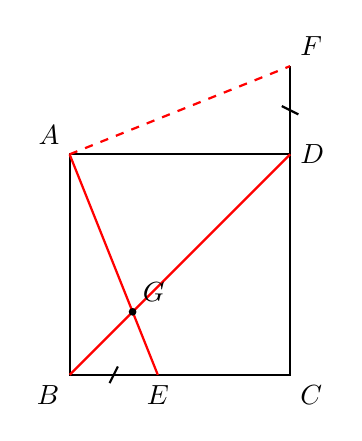
\begin{tikzpicture}[scale=1.4, thick,
  tick/.style={postaction={decorate, decoration={markings,
    mark=at position 0.5 with {\draw (-1.5pt,-3pt) -- (1.5pt,3pt);}}}}]

  \coordinate (A) at (0,2);
  \coordinate (B) at (0,0);
  \coordinate (C) at (2,0);
  \coordinate (D) at (2,2);
  \coordinate (E) at (0.8,0);    % BE = 0.8
  \coordinate (F) at (2,2.8);    % DF = 0.8 上方延长线
  \coordinate (G) at (4/7,4/7);  % AE ∩ BD

  % 正方形
  \draw (A) -- (B) -- (C) -- (D) -- cycle;
  % CD 的延长线（虚线表示延长部分）
  \draw[gray, dashed] (D) -- (F);

  % 等长边记号 BE=DF
  \draw[tick] (B) -- (E);
  \draw[tick] (D) -- (F);

  % AE 与 BD
  \draw[red] (A) -- (E);
  \draw[red] (B) -- (D);
  % 辅助线 AF
  \draw[red, dashed] (A) -- (F);

  \fill (G) circle (1.0pt);

  \node[above left]  at (A) {$A$};
  \node[below left]  at (B) {$B$};
  \node[below right] at (C) {$C$};
  \node[right]       at (D) {$D$};
  \node[below]       at (E) {$E$};
  \node[above right] at (F) {$F$};
  \node[above right] at (G) {$G$};
\end{tikzpicture}
\end{document}
